\subsubsection{Kirchhoffs lov om strømmer}
Summen av strømmene rundt et knutepunkt er null.
Eller sagt annerledes, summen av strømmene inn
er lik summen av strømmene ut.
\\
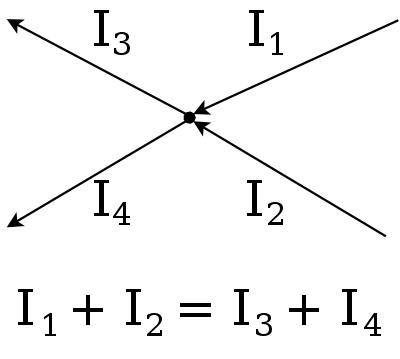
\includegraphics[width=0.25\textwidth]{./img/kcl}



\subsubsection{Kirchhoffs lov om spenninger}
Summen av alle spenninger i en krets er null.
\\
$V_{batteri} = V_1 + V_2 + V_3$
\\
\begin{circuitikz} \draw
(0,0) -- (0,1)
      to[R, l=$R_1$] (2,1)
      to[R, l=$R_2$] (4,1)
      to[R, l=$R_3$] (6,1)
      -- (6,0)
      to[battery, l=$V_{batteri}$] (0,0)
      ;
\end{circuitikz}



\subsubsection{Spenningsdeler}
Vi ser på tilfellet med to motstander seriekoblet til et batteri.
\\
\begin{circuitikz} \draw
(0,0) to[battery, l=$V_{batteri}$] (0,4)
      -- (4,4)
      to[R, l=$R_2$] (4,2)
      to[R, l=$R_1$] (4,0)
      -- (0,0)
      ;
\end{circuitikz}
\\
Hva er spenningen $V_1$ over motstanden $R_1$?
$$V_1 = \frac{R_1}{R_1 + R_2} \cdot V_{batteri}$$

Du kan tenke på det som dette:
\\
Hvor stor del av kaka tar $R_1$?
sin rettferdige andel: $\frac{R_1}{R_1 + R_2}$
\\
Hvor mye kake er det egentlig? $V_{batteri}$
